\problemname{Maskrosor}
\noindent

Under sina ungdomsdagar var Gösta helt förtjust i maskrosläsk. Tyvärr är den inte alls populär längre. 
På äldre dagar har Gösta blivit rik, och han vill nu använda sin förmögenhet för att öppna ett företag
som säljer maskrosläsk. För att göra detta kommer han självklart behöva en massa maskrosor. Han har en
äng som är $R \times C$ kvadratmeter stor. Det är välkänt att maskrosor inte trivs om de växer tätt
intill varandra. Mer exakt, om man delar upp ängen i rutor av storlek $1 \times 1$ meter, så kan det växa
som mest en maskrosa innanför varje.

Just nu växer det maskrosor på $N$ stycken celler. Gösta vill att hans äng ska ha en maskrosa i varje ruta. 
En gång om året blommar maskrosorna, och han kan då använda en stor fläkt för att blåsa antingen från väst,
öst, norr eller syd. Varje blommande maskrosas frön kommer då att röra sig en ruta i riktningen av vinden.
Om rutan den landar på är tom kommer det växa en maskrosa på den nästa år. Om det redan finns en maskrosa
på en ruta kommer den finnas kvar nästa år också. Eftersom Gösta inte har så många år kvar vill han
beräkna antalet år det tar att fylla hela ängen med maskrosor om han väljer vindriktningarna optimalt.

\section*{Indata}
Den första raden innehåller heltalen $R$ och $C$ ($1 \leq R,C \leq 10^9$), antalet rader och kolumner i rutnätet.

Därefter följer en rad med heltalet $N$ ($1 \leq N \leq 300$), antalet maskrosor i ängen just nu.

De kommande $N$ radera innehåller heltalen $r_i$ och $c_i$ ($1 \leq r_i \leq R$, $1 \leq c_i \leq C$), vilket betyder
att det till en början växer en maskros i cellen ($r_i, c_i$). I början växer aldrig två maskrosor på samma ruta.

\section*{Utdata}
Skriv ut ett heltal: det minsta antalet år för att fylla hela ängen med maskrosor om vindriktningarna väljs optimalt.

\section*{Poängsättning}
Din lösning kommer att testas på en mängd testfallsgrupper.
För att få poäng för en grupp så måste du klara alla testfall i gruppen.

\noindent
\begin{tabular}{| l | l | p{12cm} |}
  \hline
  \textbf{Grupp} & \textbf{Poäng} & \textbf{Gränser} \\ \hline
  $1$    & $5$          & $R,C \leq 4$  \\ \hline
  $2$    & $10$         & $R,C \leq 40$ \\ \hline
  $3$    & $15$         & $R \leq 40$ \\ \hline
  $4$    & $30$         & $N \leq 25$ \\ \hline
  $5$    & $20$         & $N \leq 100$ \\ \hline
  $6$    & $20$         & Inga ytterligare begränsningar. \\ \hline
\end{tabular}

\section*{Förklaring av exempelfall 1:}
Till en början finns maskrosor på följande rutor:
\begin{centering}
  \begin{figure}[h]
      \centering
      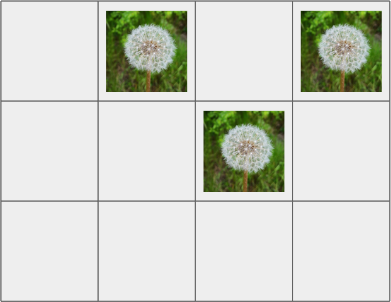
\includegraphics[width=0.8\textwidth]{t0.png}
  \end{figure}
\end{centering}
Om vi blåser vind från söder sprids maskrosorna till västerut:
\begin{centering}
  \begin{figure}[h]
      \centering
      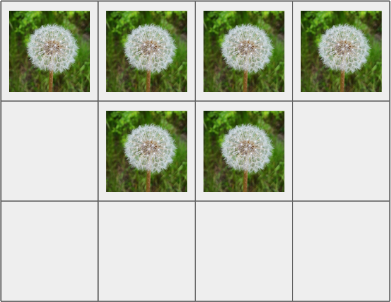
\includegraphics[width=0.8\textwidth]{t1.png}
  \end{figure}
\end{centering}
Om vi sedan blåser vind från norr sprids maskrosorna söderut:
\begin{centering}
  \begin{figure}[h]
      \centering
      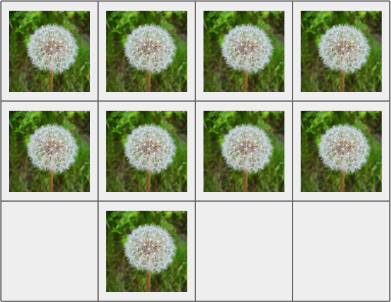
\includegraphics[width=0.8\textwidth]{t2.png}
  \end{figure}
\end{centering}
Om vi blåser från norr ännu en gång fylls hela ängen:
\begin{centering}
  \begin{figure}[h]
      \centering
      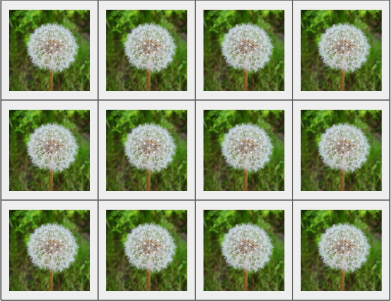
\includegraphics[width=0.8\textwidth]{t3.png}
  \end{figure}
\end{centering}
